\documentclass[a4paper, 12pt]{article}
\usepackage[a4paper,top=1.5cm, bottom=1.5cm, left=1cm, right=1cm]{geometry}
\usepackage{cmap}					
\usepackage{mathtext} 				
\usepackage[T2A]{fontenc}			
\usepackage[utf8]{inputenc}			
\usepackage[english,russian]{babel}
\usepackage{multirow}
\usepackage{graphicx}
\usepackage{wrapfig}
\usepackage{tabularx}
\usepackage{float}
\usepackage{longtable}
\usepackage{hyperref}
\hypersetup{colorlinks=true,urlcolor=blue}
\usepackage[rgb]{xcolor}
\usepackage{amsmath,amsfonts,amssymb,amsthm,mathtools} 
\usepackage{icomma} 
\usepackage{euscript}
\usepackage{mathrsfs}
\usepackage{enumerate}
\usepackage{caption}
\usepackage{enumerate}
\mathtoolsset{showonlyrefs=true}
\usepackage{graphicx}
\usepackage{caption}
\usepackage{subcaption}
\usepackage{amsthm}
\usepackage[europeanresistors, americaninductors]{circuitikz}
\DeclareMathOperator{\sgn}{\mathop{sgn}}
\newcommand*{\hm}[1]{#1\nobreak\discretionary{}
	{\hbox{$\mathsurround=0pt #1$}}{}}

\newcommand{\framedtext}[1]{%
\par%
\noindent\fbox{%
    \parbox{\dimexpr\linewidth-2\fboxsep-2\fboxrule}{#1}%
}%
}

\title{\textbf{Измерение коэффициента поверхностного натяжения жидкости (2.5.1)}}
\author{Манро Эйден}
\date{}

\begin{document}

\maketitle

\begin{center}
    \section*{Введение}
\end{center}

\noindent \textbf{Цель работы:} 1) измерение температурной зависимости  коэффициента поверхностного натяжения дистиллированной воды с использованием известного коэффициента поверхностного натяжения спирта; 2) определение полной поверхностной энергии  и теплоты, необходимой для изотермического образования единицы поверхности жидкости  при различной температуре.

\bigskip

\noindent \textbf{Оборудование:} прибор  Ребиндера  с термостатом и микроманометром; исследуемые жидкости; стаканы.

\bigskip

\begin{center}
    \subsection*{Теоретические сведения}
\end{center}

Наличие поверхностного слоя приводит к разнице давлений по разные стороны от искривленной границы раздела двух сред. 
Для сферического пузырька с воздухом внутри жидкости избыточное давление рассчитывается с использованием формулы Лапласа,

\begin{equation} \label{laplas}
    \Delta P = \frac{2\sigma}{r}
\end{equation}

где $\sigma$  – коэффициент поверхностного натяжения, $P_{\text{внутри}}$ и $P_{\text{снаружи}}$ – давление внутри пузырька и снаружи, $r$ – радиус кривизны поверхности раздела двух фаз. Эта формула является основой предложенного метода определения коэффициента поверхностного натяжения жидкости. Для этого измеряется давление $\varDelta P$, необходимое для выталкивания в жидкость пузырька воздуха.

\begin{center}
    \subsection*{Экспериментальная установка}
\end{center}

\begin{figure}[H] 
    \center{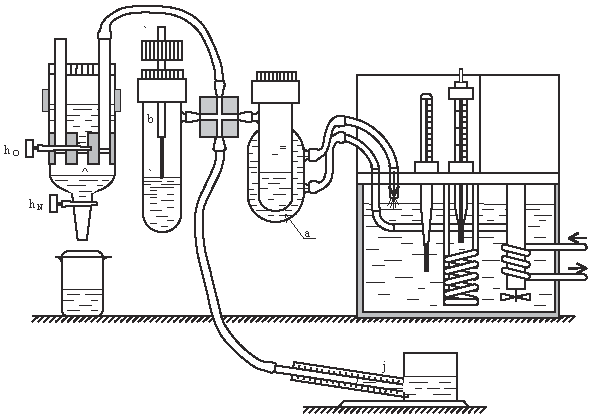
\includegraphics[scale=1]{img/ustanovka.pdf}}
    \caption{Схема установки для измерения температурной зависимости коэффициента поверхностного натяжения.}
    \label{ris:ustanovka}
\end{figure}

Исследуемая жидкость (дистиллированная вода) наливается в сосуд (колбу) \textbf{В} (рис. \ref{ris:ustanovka}). Тестовая жидкость  (этиловый спирт) наливается  в сосуд \textbf{E}. При измерениях  колбы герметично закрываются  пробками.   Через одну из двух пробок  проходит полая металлическая игла \textbf{C}. Этой пробкой закрывается сосуд, в котором  проводятся измерения. Верхний конец иглы открыт в атмосферу, а нижний погружен в жидкость. Другой сосуд герметично закрывается второй пробкой. При создании достаточного  разряжения воздуха в колбе с иглой пузырьки воздуха начинают пробулькивать через жидкость. Поверхностное натяжение можно определить по величине разряжения $\Delta P$ (\ref{laplas}), необходимого для прохождения пузырьков (при известном радиусе иглы).\\
Разряжение в системе создается с помощью аспиратора \textbf{A}. Кран \textbf{K2} разделяет две полости аспиратора. Верхняя полость при закрытом кране \textbf{K2}  заполняется водой. Затем кран \textbf{K2} открывают и заполняют водой  нижнюю полость  аспиратора.  Разряжение воздуха создается в нижней полости  при открывании крана \textbf{K1}, когда  вода вытекает из неё по каплям. В колбах \textbf{B} и \textbf{C}, соединённых трубками с нижней полостью аспиратора,  создается такое же пониженное давление. Разность давлений в полостях с разряженным воздухом и атмосферой измеряется спиртовым микроманометром.

\bigskip

\begin{center}
    \subsection*{Погрешности}
\end{center}

\begin{center}
    \item $\sigma_{\text{микроскоп}} = 0,05 \; \text{мм}$ \; $\sigma_{\text{линейка}} = 0,5 \; \text{мм}$ \; $\sigma_{\text{манометр}} = 0,1 \; \text{Па} $ 
\end{center}

    
\newpage


\begin{center}
    \section*{Ход работы}
\end{center}

\subparagraph{1.} Проверим герметичность установки. 

\subparagraph{2.} Откроем кран К1. Подберём частоту падения капель около одной капли в 5 секунд. 

\subparagraph{3.} Измерим максимальное давление $\Delta P_{\text{спирт}}$  при  пробулькивании пузырьков воздуха через спирт. Данные занесём в таблицу 1. По разбросу результатов оценим случайную погрешность измерения. 

\begin{table}[h!]
    \centering
    \begin{tabular}{|c|c|c|c|c|c|c|c|c|c|c|} \hline

        $N$             & 1  & 2  & 3  & 4  & 5  & 6  & 7  & 8  & 9  & 10  \\ \hline
        $h$, \text{дел} & 46 & 45 & 46 & 45 & 45 & 45 & 45 & 45 & 45 & 45  \\ \hline
        \multicolumn{11}{|l|}{$h_{\text{ср}} = 45,2$ \text{дел} \hspace{125} $\sigma_h = 0,3$ \text{дел}} \\ \hline
        
    \end{tabular}
    \caption{Измерения для спирта ($h_{\text{сп}}$)}
\end{table}

В таблице учтена только случайная погрешность величины $h$, которая составляет около $0,7 \; \%$  в то время как приборная погрешность составляет две цены деления (1 деление -- инструментальная погрешность и плюс ещё одно -- моя реакция и способность зафиксировать правильное деление), то есть её относительный вклад $\approx 2 / 46   \approx 4.3\%$.

\bigskip

По формуле $\Delta P_{\text{спирт}} = 0.2 \cdot 9.81 \cdot h$ вычислим $\Delta P_{\text{спирт}}$.

\bigskip

\begin{center}
    \underline{ $\Delta P_{\text{спирт}} = (88.7\pm 3.8) \; \text{Па}$}
\end{center}

Пользуясь табличным значением коэффициента поверхностного натяжения спирта, определим по формуле (1) диаметр иглы. 

\begin{itemize}
    \item 
    $
    \sigma_{\text{спирт, табл.}} = 22,4 \cdot 10^{-3} \; \frac{\text{Дж}}{\text{м}^2}.
    $
    
    \item 
    $
    d_{\text{рассч.}}= \dfrac{4\sigma_{\text{спирт, табл.}}}{\Delta P_{\text{спирт}}}\approx 1.01~\text{мм}.
    $
    
    \item 
    $
    \dfrac{\sigma_d}{d}=\sqrt{\left(\dfrac{\sigma_{\Delta P}}{\Delta P}\right)^2}\approx 4.3\%.
    $
\end{itemize}

\bigskip
    
Тогда итоговое значение:

\begin{center}
    $
    \underline{d_{\text{рассч.}} = (1.01 \pm 0.05) \; \text{мм}}.
    $
\end{center}

Теперь воспользуемся микроскопом чтобы измерить диаметр иглы и сравним его с рассчитанным.
 
\begin{center}
$
\underline{d_{\text{изм.}} = (1.00 \pm 0.05) \; \text{мм}}.
$
\end{center}

Как видно, в пределах погрешности величины диаметра иглы совпали, что говорит о хорошо проведённых измерениях. 

\subparagraph{4.} Теперь перенесём иглу в колбу с водой, предварительно промыв её. Измерим максимальное давление $P_1$ при пробулькивании пузырьков, когда игла лишь касается поверхности воды. Отрегулируем скорость поднятия уровня спирта в манометре (около одной капли в 5 секунд) и будем сохранять её в течение всех экспериментов. 

\begin{table}[H]
    \centering
    \begin{tabular}{|c|c|c|c|c|c|c|c|c|c|c|} \hline

        $N$             & 1  & 2  & 3  & 4  & 5  & 6  & 7  & 8  & 9  & 10  \\ \hline
        $h$, \text{дел} & 138 & 137 & 137 & 137 & 138 & 137 & 137 & 137 & 137 & 137  \\ \hline
        \multicolumn{11}{|l|}{$h_{\text{ср}} = 137,2$ \text{дел} \hspace{175} $\sigma_h = 0,4$ \text{дел}} \\ \hline
        
    \end{tabular}
    \caption{Измерения для воды ($h_{\text{сп}}$)}
\end{table}

Аналогично п.3 основной вклад в погрешность величины $h$ определяется инструментальной погрешностью, которая равна $\approx 2 / 137 \approx  1.5 \% $. Аналогично п.3 вычислим давление и в результате получим:

\begin{center}
$
\underline{P_1 = (268.8 \pm 4.0) \; \text{Па}}.
$
\end{center}
    
Измерим расстояние между верхним концом иглы и любой неподвижной частью прибора $h_1$.

\begin{center}
$
\underline{h_1 = (2.70 \pm 0.05) \; \text{см}}.
$
\end{center}

\subparagraph*{5.} Утопим иглу до предела. Аналогично п.4 измерим $h_2$ и $P_2$.


\begin{table}[H]
    \centering
    \begin{tabular}{|c|c|c|c|c|c|c|c|c|c|c|} \hline

        $N$             & 1  & 2  & 3  & 4  & 5  & 6  & 7  & 8  & 9  & 10  \\ \hline
        $h$, \text{дел} & 230 & 229 & 229 & 229 & 229 & 229 & 229 & 229 & 229 & 230  \\ \hline
        \multicolumn{11}{|l|}{$h_{\text{ср}} = 239,2$ \text{дел} \hspace{175} $\sigma_h = 0,4$ \text{дел}} \\ \hline
        
    \end{tabular}
    \caption{Измерения давления $P_2$}
\end{table}
\begin{center}
$
\underline{P_2 = (469.3 \pm 3.9) \; \text{Па}}.
$  
\end{center}

\begin{center}
$
\underline{h_2 = (0.60 \pm 0.05) \; \text{см}}.
$
\end{center}

По разности давлений $\Delta P= P_2 - P_1$ определим глубину погружения $\Delta h_1$ иглы и сравним с $\Delta h_2 =  h_1- h_2$. Погрешности при этом получаются по формулам $\frac{\sigma_{\Delta h_1} }{\Delta h_1}= \sqrt{\left(\frac{\sigma_{P_1}}{P_1}\right)^2 + \left(\frac{\sigma_{P_2}}{P_2}\right)^2}$ и $\frac{\sigma_{\Delta h_2} }{\Delta h_2}= \sqrt{\left(\frac{\sigma_{h_1}}{h_1}\right)^2 + \left(\frac{\sigma_{h_2}}{h_2}\right)^2}$

\begin{center}
    
$
\underline{\Delta h_2 = h_1 - h_2 = (2.10 \pm 0.08) \; \text{см}}.
$
    
\end{center}

\begin{center}
    
$
\underline{\Delta h_1 = \dfrac{P_2 - P_1}{\rho g} = (2.04 \pm 0.06) \; \text{см}}. 
$

\end{center}

Полученные значения для глубины погружения сходятся, соответственно все было грамотно измерено.

\subparagraph{6.} Снимем температурную зависимость $h (T)$ дистиллированной воды. Для этого включим термостат и подождём, пока нужная нам температура не стабилизируется. После этого проведём измерение давления. И так будем снимать показания через каждые 3 градуса. Результаты измерений занесены в Таблицу 4. 


\begin{table}[H]
	\caption{Измерение давления в зависимости от температуры}
	\centering 
	\begin{tabular}{{|l}*{13}{|l}} \hline 
		$T,~^\circ C$ & \multicolumn{10}{c|}{$h, \; \text{дел}$}& $h_{\text{ср}}, \; \text{дел} $& $ \sigma_h, \; \text{дел}$\\ \hline
		23,5 & 230 & 229 & 229 & 229 & 229 & 229 & 229 & 229 & 229 & 230 & 229,2 & 0,17 \\ \hline 
		28,9 & 228 & 228 & 228 & 228 & 227 & 227 & 227 & 227 & 227 & 227 & 227,4 & 0,26 \\ \hline
		34,4 & 227 & 227 & 227 & 227 & 226 & 226 & 226 & 226 & 226 & 227 & 226,5 & 0,27 \\ \hline 
		39,5 & 225 & 225 & 225 & 225 & 225 & 224 & 224 & 224 & 225 & 225 & 224,7 & 0,23 \\ \hline
		45,2 & 224 & 224 & 224 & 224 & 224 & 224 & 223 & 223 & 223 & 223 & 223,6 & 0,26 \\ \hline 
		50,1 & 223 & 222 & 222 & 223 & 223 & 222 & 222 & 222 & 222 & 222 & 222,3 & 0,23 \\ \hline
		55,1 & 221 & 221 & 221 & 221 & 221 & 221 & 220 & 220 & 220 & 220 & 220,6 & 0,26 \\ \hline 
        59,0 & 219 & 219 & 219 & 219 & 219 & 219 & 218 & 218 & 218 & 218 & 218,6 & 0,26 \\ \hline 

	\end{tabular}
\end{table}

\subparagraph*{7.} Оценим погрешность измерения давления и температуры. Для давления погрешность вычисляется аналогично п.3, а температура измерена с точностью около $0.2 \; ^\circ C$, что составляет около $0.1 \%$, поэтому данная погрешность учитываться не будет ввиду её малости рассчитаем величину коэффициента поверхностного натяжения воды  $\sigma$, используя формулу, которая следует из (1): 

\begin{center}
    $
    \frac{\Delta P_{\text{сп}}}{\Delta P} = \frac{\sigma_{\text{сп}}}{\sigma} .
    $
\end{center}

\bigskip

Поскольку $P \propto h,$ то для вычисления $\sigma$ возьмём $h$ из Таблиц 1 и 2. При этом относительная погрешность величины $\sigma$  складывается из относительных погрешностей измерения давления: $\varepsilon_\sigma =\sqrt{\varepsilon_{h_1}^2 + \varepsilon_{h_2}^2} \approx 4.4 \%$, в результате чего получаем: 

\bigskip

$
\sigma = \sigma_{\text{сп}}\dfrac{h}{h_{\text{сп}}} \approx (67,9 \pm 3,0)\cdot 10^{-3} \; \frac{\text{Дж}}{\text{м}^2}.
$

\bigskip

В то время как табличное значение коэффициента поверхностного натяжения воды при $25^\circ C$ составляет $71.8 \cdot 10^{-3} \; \frac{\text{Дж}}{\text{м}^2}, $ что почти перекрывается с полученным нами значением. 

\subparagraph*{8.}По данным Таблицы 4 построим график зависимости  $h(T)$ (Рис. 2).


Используя МНК определим коэффициент наклона $\underline{k = -0,28 \; \frac{\text{дел}}{^\circ C}}$. 
Определим по графику температурный коэффициент:

\begin{center}
    $\alpha = - \dfrac{d\sigma}{dT} = -\dfrac{\sigma_{\text{сп}}}{h_{\text{сп}}}\cdot \dfrac{d h}{d T} = -\dfrac{\sigma_{\text{сп}}}{h_{\text{сп}}}\cdot k \approx \underline{0,14 \; \frac{\text{мДж}}{\text{м}^2}} \cdot K$. 
\end{center}  
 
Оценим точность результата. Пренебрежём погрешностью, вносимой инструментальной погрешностью термометра (почему это можно сделать описано ранее), поэтому итоговая погрешность величины складывается из погрешности, возникающей из-за аппроксимацией прямой (вычисляется по формуле из МНК $\sigma_k = \frac{1}{\sqrt{n}}\sqrt{\frac{\left< h^2\right>}{\left< t^2\right>} - k^2} \approx 0.04 \frac{\text{мДж}}{\text{м}^2} \; \cdot K,$  то есть $\varepsilon_k =  12 \%$) Поскольку величина $h$ измерена с точностью не менее $4\%$ (по оценкам выше), то будем учитывать вклад только погрешности, возникающей из МНК. Тогда итоговый результат:


\begin{center}
    $
    \underline{\alpha = ( 1,40 \pm 0,18)  \cdot 10^{-4} \; \frac{\text{Дж}}{\text{м}^2} \cdot K}.
    $
\end{center}

Это значение перекрывается с табличным $1.54 \cdot 10^{-4} \; \frac{\text{Дж}}{\text{м}^2} \cdot K$ в пределах погрешности. 

\subparagraph*{9.}На других графиках построим зависимость от температуры 


а) теплоты образования единицы поверхности жидкости $q=-T\dfrac{d\sigma}{dt} = \alpha T$ (Рис. 4) 






б) поверхностной энергии $U$ единицы площади $F:   \dfrac{U}{F}= \sigma - T\dfrac{d\sigma}{dT}$ (Рис. 5). 

\begin{figure} [H]
	\centering 
	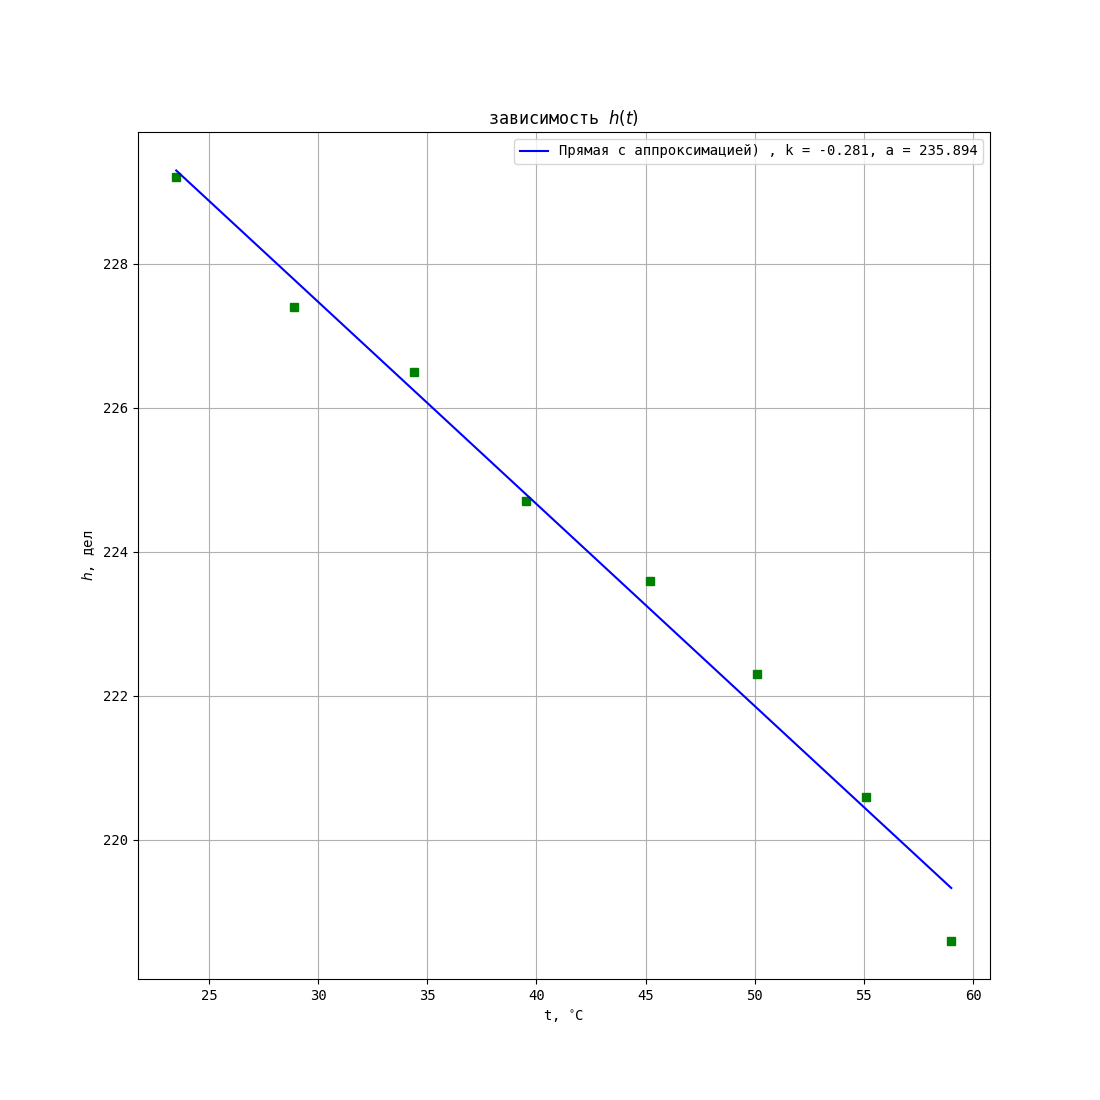
\includegraphics[scale=0.55]{img/h(t).png} 
	\caption{График, демонстрирующий измеренную зависимость давления от температуры} 
\end{figure}

\end{document}